\section{Functional Requirements}

\subsection{Program Workflow}
\label{sec:program_workflow}
To aid the development of the functional requirements, the program workflow was
charted in order to give a better understanding of what the system was expected
to do. This was accomplished by going through the functionality of \bhtb{} with
Avdeling BKI and detailing the functions and various needs for improvement or
additional functionality. From this, a workflow chart (Figure
\ref{fig:program_workflow}) was drawn with the major parts of the system. In addition, Henriksen's management process \cite{BHTB} was taken into consideration.

\begin{figure}[ht!]
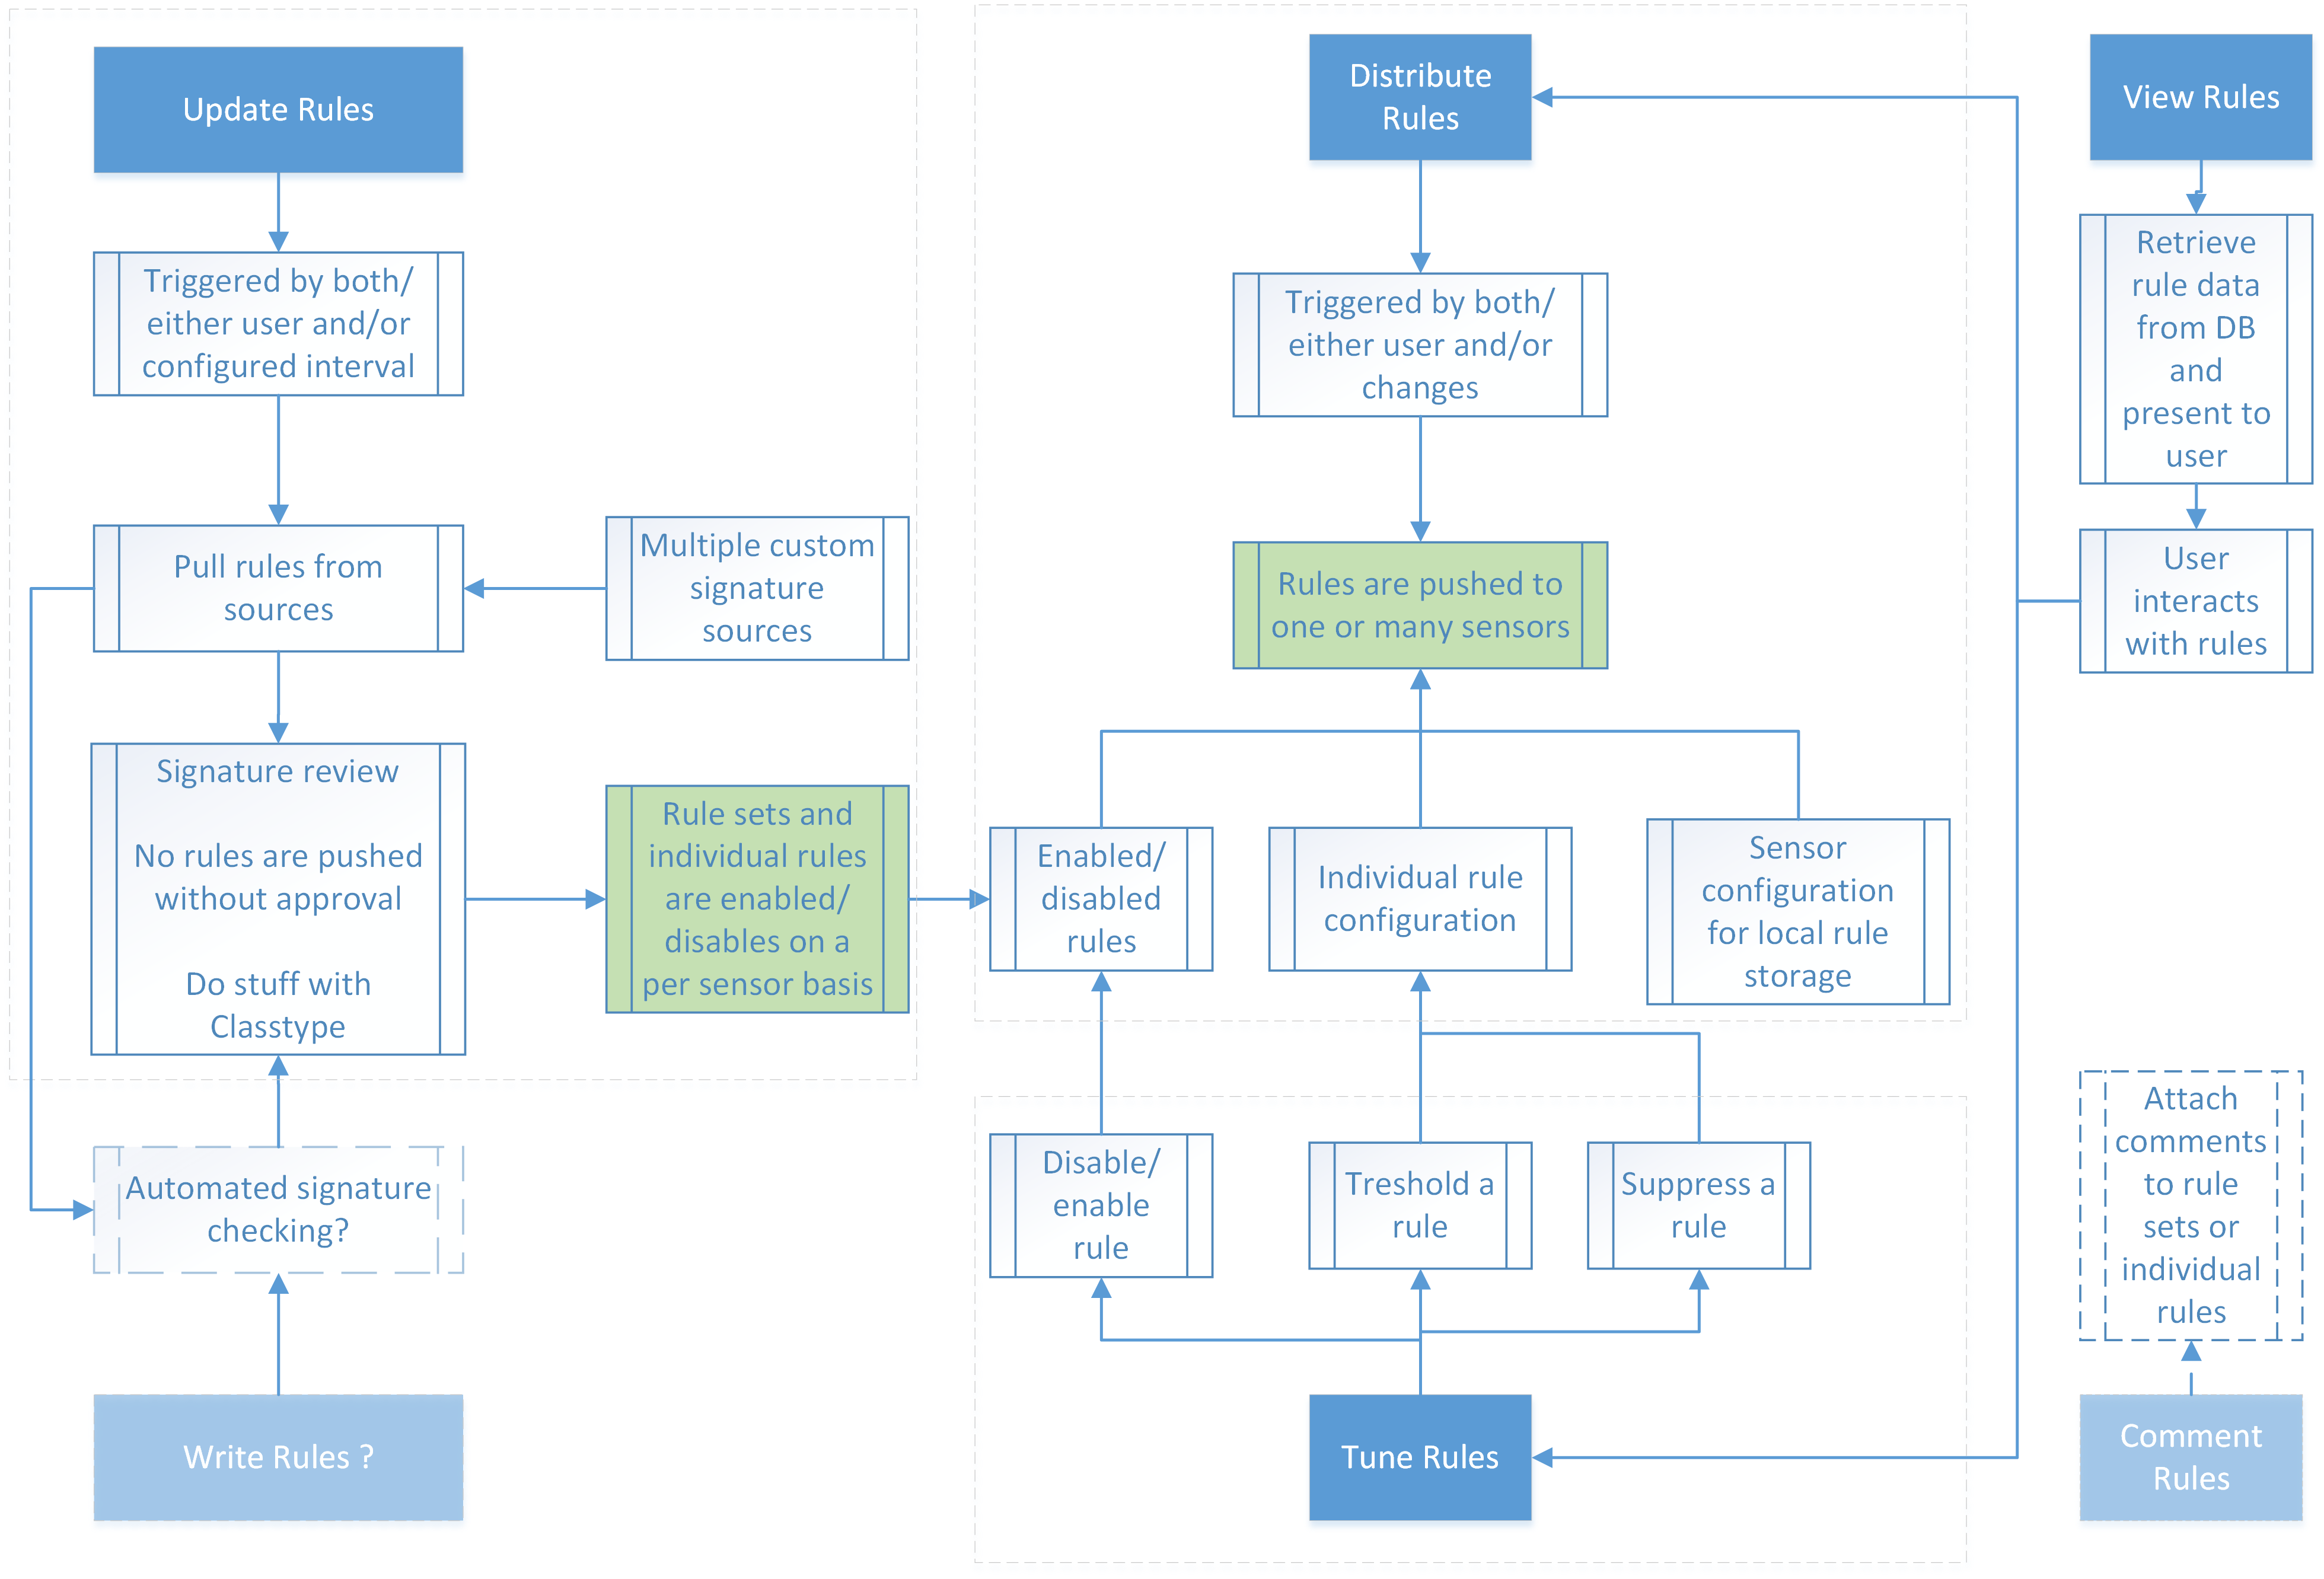
\includegraphics[width=200mm,angle=90]{./img/program_workflow_v2.png}
\caption{Program workflow}
\label{fig:program_workflow}
\end{figure}

To explain the workflow chart in Figure \ref{fig:program_workflow}: the blue
boxes are the major system functionalities, the green boxes are the major goals
of the system and the arrows show the direction of flow the system should have.
As can be seen, all of the program flow ends up with rules being synchronised to
the sensors, making that a very central part of the system. It is important to
note that in the beginning of the development, we decided that writing rules,
automatically check for errors and adding user comments to them were
nice-to-have (but still important) features that we could implement if we had
time to do so. Hence, they are greyed out in the drawings, and left for future work.

From the workflow we could outline a rough modular design (figure
\ref{fig:program_modules}) based on the naturally separate functions of updating
rules, tuning them, distributing them and showing them. We also added a database
module, since most of our program was going to be centered around it.

\begin{figure}[!p]
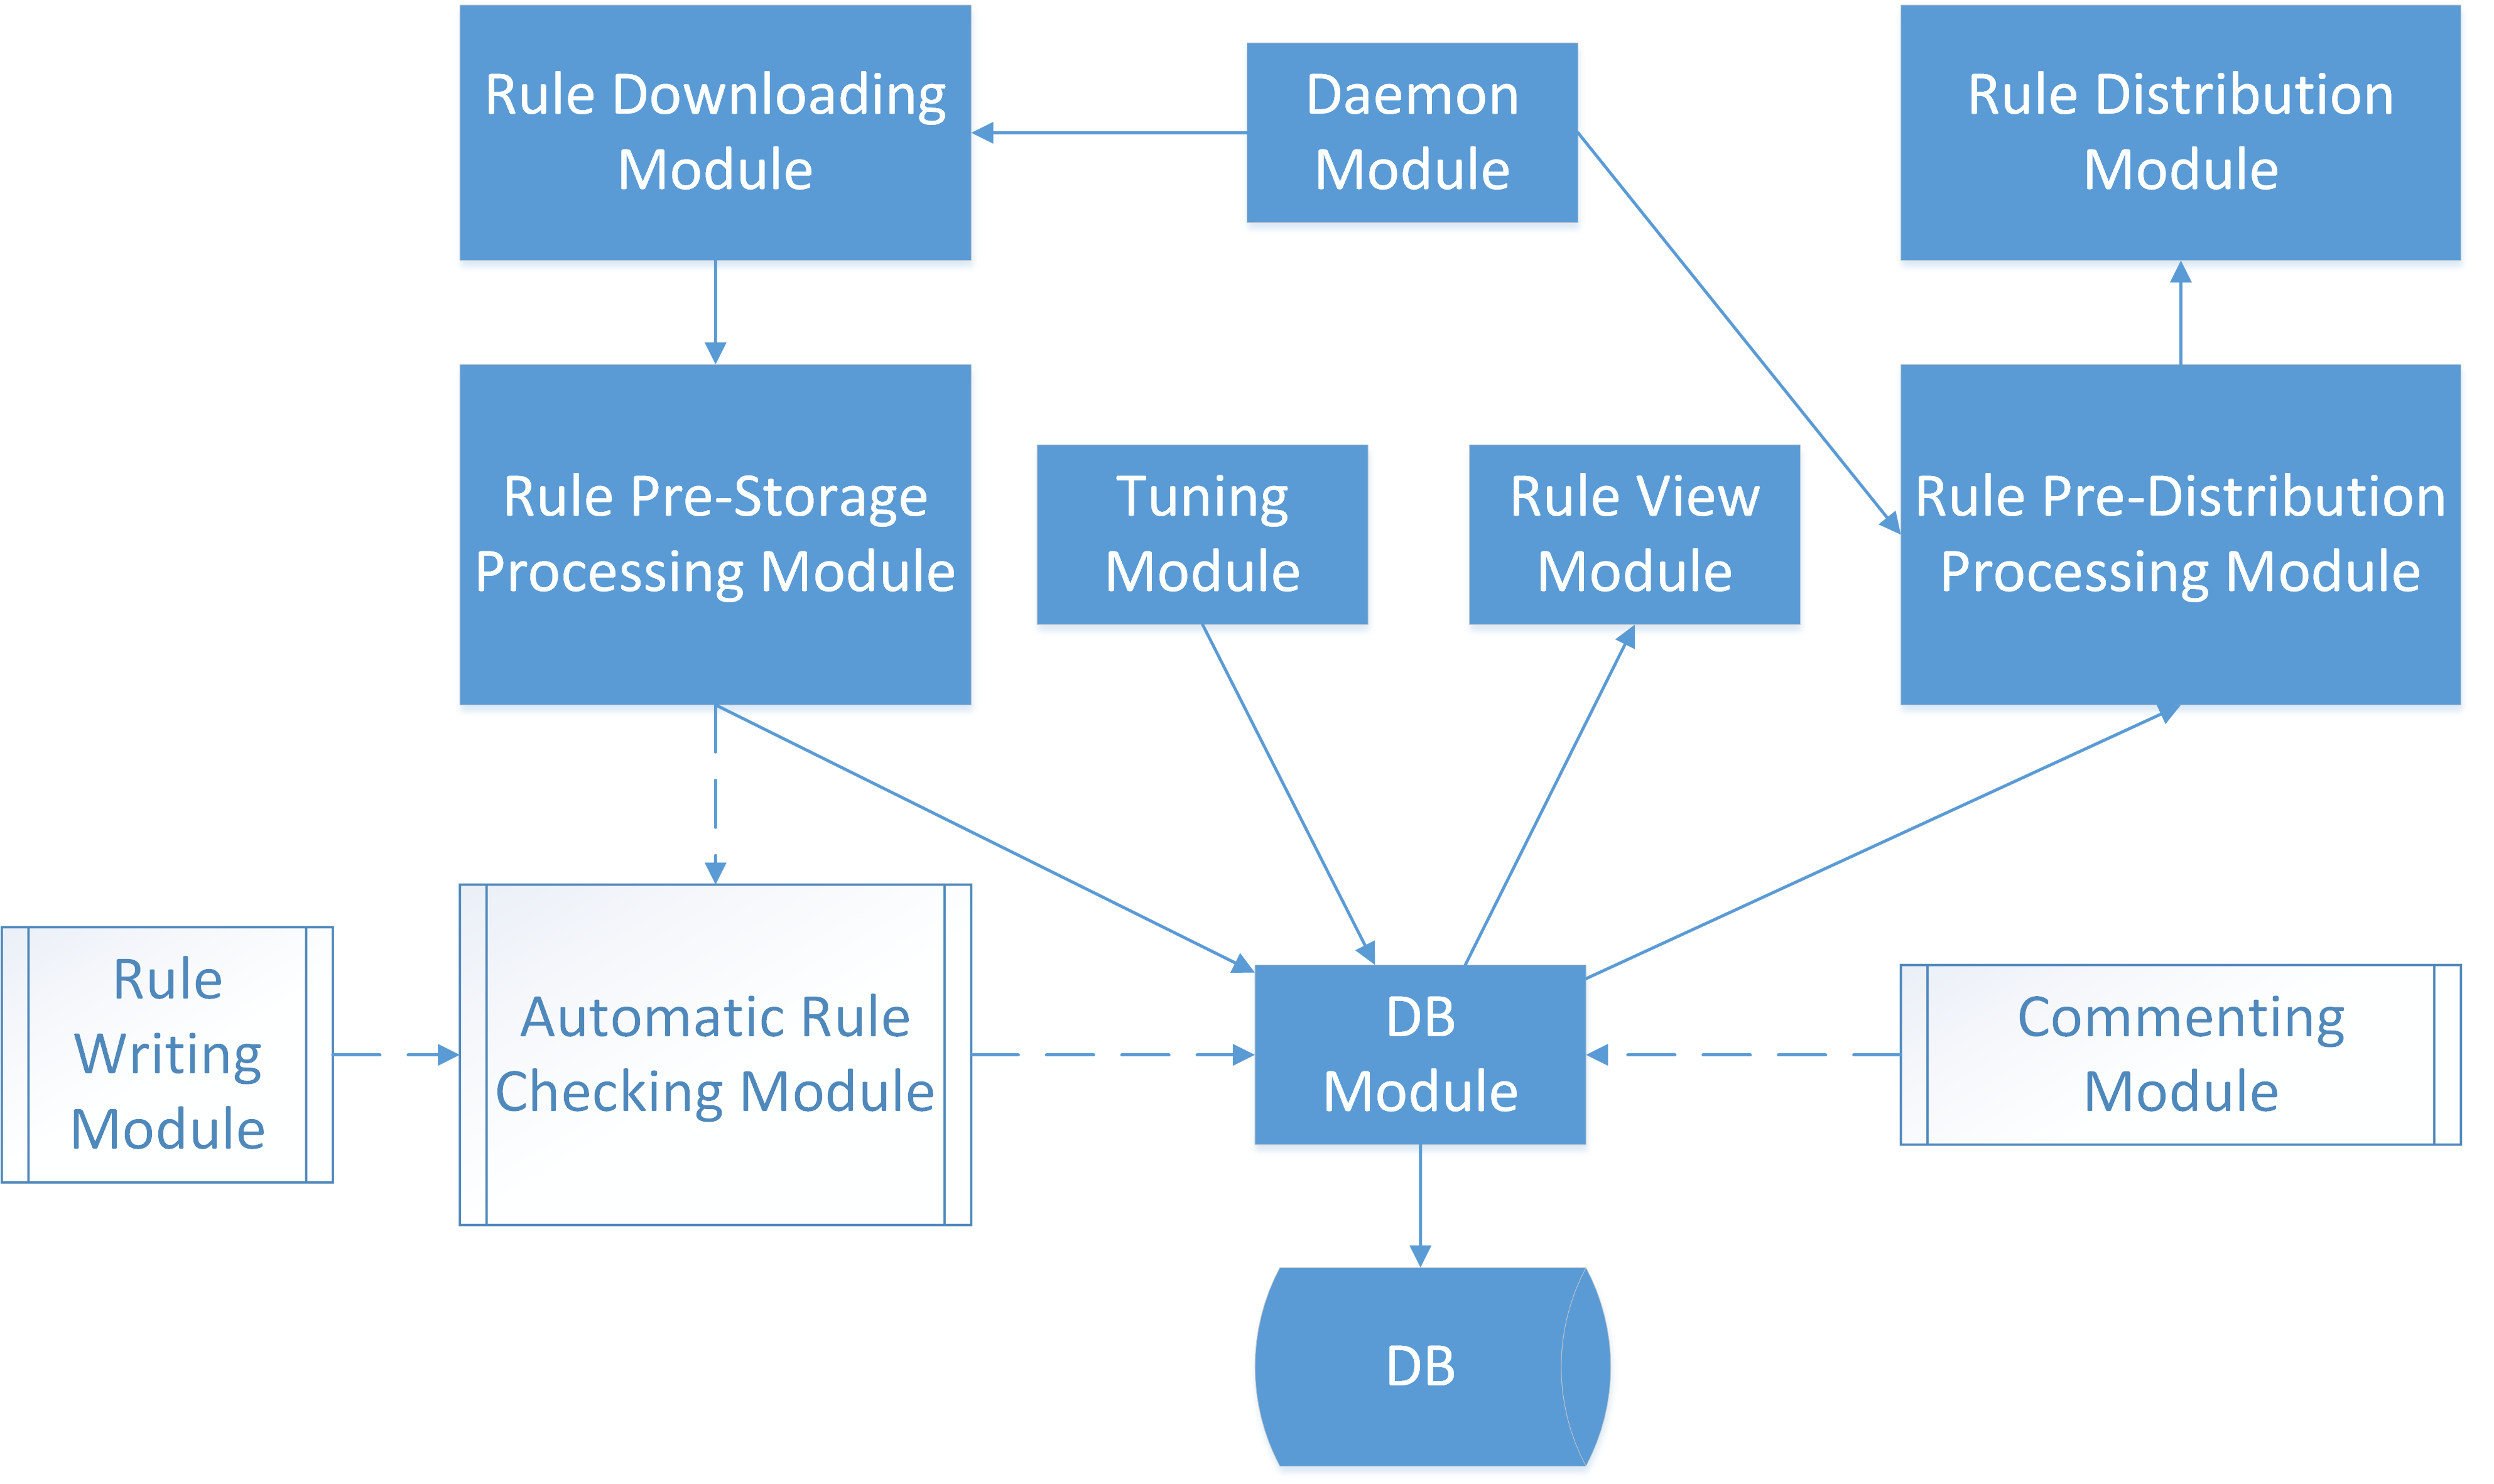
\includegraphics[width=200mm,angle=90]{./img/program_modules_v2.png}
\caption{Program modules}
\label{fig:program_modules}
\end{figure}

\subsubsection{Rule download module}
This module will handle all functionality related to downloading rules,
including comparing MD5 checksums.
\subsubsection{Rule pre-storage processing module}
This module will essentially take downloaded rules, and parse and process them
into objects that can be fed into the database.
\subsubsection{DB Module}
This module will handle all input and output to/from the database.
\subsubsection{Rule pre-distribution processing module}
This module will essentially take rules stored in the database and prepare them for
distribution to sensors.
\subsubsection{Rule distribution module}
This module will be in charge of distributing rules out to the \snort{} sensors
and handing the rules over to \snort{} itself.
\subsubsection{Tuning module}
This module will handle all functionality related to turning rules on or off,
filtering them or suppressing them.
\subsubsection{Rule view module}
This module will contain all the functionality needed to display the system
status and system functions to the user. It will be the primary way the user
interacts with the system, and thus contain the GUI.
\subsubsection{Daemon module}
This module will run continuously on the system to ensure that the system is
responsive and to carry out any timed tasks, such as automatic updates or
automatic distributions.
\subsubsection{Commenting module}
This module will allow users to attach comments to rules.
\subsubsection{Rule writing module}
This module will handle functionality for writing custom rules and editing existing rules.
\subsubsection{Automatic rule checking module}
This module will be responsible for verifying rules to ensure that there are no malformed or
misconfigured rules that may potentially break or cause a halt on a Snort
sensor.

\subsection{High Level Use Cases}
Looking at the arrows in program workflow figures, it is pretty apparent that
the program workflow is heavily centered around the database module, and the
major parts of the system revolves around the importing of rules and then distributing them. We therefore began developing our use cases around those major movements.

We've added the most central use cases for this system below, but additional use
cases is available in appendix B.


%OK
\begin{usecase}
\addtitle{Use case}{Manual rule update}
\addfield{Primary actor}{User}
\addfield{Purpose}{Update the central rule database with the newest rules and 
revisions.} \addfield{Description}{The user commands the server to update the rules, either from a local file or from external sources. When the latter is the case, the server pulls rule files from all the sources specified in the list of
sources. In both cases rules are processed and stored in the database.}
\addfield{Preconditions}{Either a file or one or more sources must exist.}
\addfield{Postconditions}{The central rule database is up to date with the
newest rules and revisions.}
\end{usecase}

%OK
\begin{usecase}
\addtitle{Use case}{Automatic rule update}
\addfield{Primary actor}{Daemon}
\addfield{Purpose}{Update the central rule database with the newest rules and 
revisions.}
\addfield{Description}{At configured time-intervals, the system  daemon triggers
a rule database update. The server pulls rule files from all the sources
specified in the list of sources to be updated at the given interval, processes
the rules and then stores them in the database.}
\addfield{Preconditions}{One or more sources must exist.}
\addfield{Postconditions}{The central rule database is up to date with the
newest rules and revisions}
\end{usecase}

%OK
\begin{usecase}
	\addtitle{Use case}{Manual rule distribution}
	\addfield{Primary actor}{User}
	\addfield{Purpose}{Distribute rules to sensors as per the settings in the
	database.}
	\addfield{Description}{The user sends a command to distribute rules to
	either all or specified sensors. The server then begins the distribute routine,
	and eventually all sensors will be up to date with the rules and rulesets
	they should have.}
	\addfield{Preconditions}{Rules and sensors must exist}
	\addfield{Postconditions}{Specified sensors contain rules as per settings in
	the central database.}
\end{usecase}

%OK
\begin{usecase}
	\addtitle{Use case}{Automatic rule distribution}
	\addfield{Primary actor}{Daemon}
	\addfield{Purpose}{Distribute rules to sensors as per the settings in the
	database.}
	\addfield{Description}{Configured at intervals, the system triggers a command
	to distribute rules to specified sensors. The server then begins the distribute
	routine, and eventually all sensors will be up to date with the rules and
	rulesets they should have.}
	\addfield{Preconditions}{Rules and sensors must exist}
	\addfield{Postconditions}{Specified sensors contain rules as per settings in
	the central database.}	
\end{usecase}

%OK
\begin{usecase}
	\addtitle{Use case}{Enable/Disable a rule or ruleset}
	\addfield{Primary actor}{User}
	\addfield{Purpose}{Enable or disable one or more rule or ruleset on one or more
	sensors.}
	\addfield{Description}{The user either enables or disables a rule or a ruleset
	so that the rule is either on or off on certain sensors. This status is then
	shared with the sensor and the sensor syncronizes as needed.}
	\addfield{Preconditions}{Rules and/or rulesets must exist.}
	\addfield{Postconditions}{A rule or ruleset has been modified to be enabled or
	disabled and the change is syncronized to affected sensors.}
\end{usecase}

%OK
\begin{usecase}
	\addtitle{Use case}{Set rule threshold or suppression}
	\addfield{Primary actor}{User}
	\addfield{Purpose}{Set or remove a threshold or suppression for a rule on one
	or more sensors.}
	\addfield{Description}{User sends a command with either
	thresholding/suppression parameters or removal of a threshold or suppression
	for a rule on one or more sensors. The system updates the database and distributes the change to the sensor(s).}
	\addfield{Preconditions}{Rules and sensor(s) must exist.}
	\addfield{Postconditions}{Rule tuning is saved in the central database and
	distributed to affected sensors.}
\end{usecase}

%OK
\begin{usecase}
	\addtitle{Use case}{View rules}
	\addfield{Primary actor}{User}
	\addfield{Purpose}{Display rules to the user.}
	\addfield{Description}{Rules are retrieved from the database, processed for GUI
	format and then delivered to the GUI.}
	\addfield{Preconditions}{Rules must exist.}
	\addfield{Postconditions}{The user is informed of the current status of the
	central database and the status of rules and rulesets enabled/disabled on
	sensors.}
\end{usecase}

\newpage
\subsection{Detailed Use Cases}
We also worked on some detailed use cases on our more complex system modules.
Again, more use cases are available in appendix B.

%OK, create sequence diagram
\begin{usecase}
	\addtitle{Use case}{Central rule-database update}
	\addfield{Primary actor}{Server}
	\addfield{Purpose}{Update the central rule database with the newest rules and 
revisions.}
	\addfield{Description}{
		An update can be triggered either by the user or the daemon. The system
		retrieves the files in question, checks what is new and what is not and then
		updates the database accordingly.
	}
	\addfield{Preconditions}{Depending on the request, this process requires a
	local file or the server must be configured with external source(s).}
	\addfield{Postconditions}{The central rule-database is up to date with the
	latest rules and revisions.} \addfield{Triggers}{
		Manual rule update,
		Automatic rule update,
		Write rule
	}
	\addscenario{Basic Flow:}{
		\item Update is triggered.
		\item Rule Downloading Module compares hash values from external sources with last update.
		\item Updated rule files are downloaded from sources. The files are validated
		and passed to the Pre-Storage Processing Module.
		\item The new files are parsed for rule SID and revision number. 
		\item A list of rule SID and revision numbers are gathered from the database
		and these are compared to identify which rules are new or modified.
		\item New or changed rules are then parsed into objects and
		these objects are passed to the Database/Core Module.
		\item The Database/Core Module stores the new or changed rule objects into the
		database. The user is notified that the update is complete and given a list
		of changes.
	}
	\addscenario{Extensions:}{
		\item 
		\begin{enumerate}
			\item Update is triggered by user.
			\item Update is triggered by daemon.
		\end{enumerate}
		\item 
		\begin{enumerate}
			\item The hash-values from all sources are identical with previously stored values. Database is up to date and the update process terminates. User is notified that database is up to date.
			\item The hash value from one or more sources is newer than previously stored values. Database must be updated, and the user is notified that the database is not up to date and an update process has begun.
		\end{enumerate}		
	 }
	\addscenario{Error handling:}{
		\item The source and database checksum is different but the source rules are
		older than what is stored in the database: \textit{The program can still
		continue, because if the SIDs already exist they will not be added again and if the revisions are older the rules will also not be updated.}
		\item A ruleset has changed its name or one or more rules are moved to a
		different ruleset: \textit{Based on a configuration file, the affected rules
		will either be a) automatically moved to the new ruleset or b) stay put in their
		original ruleset. The user will be notified and can choose to reverse or
		distribute the changes in either case.}
		}
\end{usecase}

%OK
\begin{usecase}
	\addtitle{Use case}{Distribute rules}
	\addfield{Primary actor}{Server}
	\addfield{Purpose}{Distribute rules from the central database to the sensors.}
	\addfield{Description}{After a command to synchronise is sent either by the
	user or the daemon, the server calculates and organizes the central database
	data and synchronizes this information with the affected sensors.}
	\addfield{Preconditions}{One or more rulesets or rules must be present in the
	central database. One or more sensors must be registered.}
	\addfield{Postconditions}{The rules on the sensor(s) are synchronized to
	reflect those in the central database that are enabled/disabled for those
	sensors.}
	\addfield{Triggers}{Manual rule distribution, Automatic rule distribution}
	\addscenario{Basic flow}{
		\item Synchronize signal is sent.
		\item The system calculates and organizes the data for each sensor affected by the synchronization.	
		\item The system initializes a synchronization protocol with the affected sensor or sensors, sending a list of what the sensor should have.	
		\item The sensor calculates diff between should have and has.
		\item Compare diff.
		\item Send update.
		\item The sensor includes the new changes into its database and files and tells the central system that it is now up to date.
		\item The system carries out maintenance to reflect the synchronization.
		\item The user is notified that all sensors affected are now up to date.			
	}
	\addscenario{Extensions}{
		\item
		\begin{enumerate}
			\item User sends a command to synchronize one, more or all sensors		
			\item The system reaches an interval for synchronizing all sensors.		
		\end{enumerate}
		\etcounter{enumi}{4}
		\item
		\begin{enumerate}
			\item The sensor content is different from what it should have, asks central system to send what it needs.
			\item The sensor content is not different from what it should have, no further action is required. This status is sent to the central system.
		\end{enumerate}	
		\item
		\begin{enumerate}
			\item The system retrieves and sends what the sensor asks for.
			\item The system terminates the synchronization protocol with the sensor in question.
		\end{enumerate}				
	}
	\addscenario{Error handling}{
		\item The change may never be synced to the sensor due to errors: \textit{There must be an error protocol that is followed in this scenario.}
	}
\end{usecase}

\subsection{Use Case Diagram}

The use case diagram is presented in Figure \ref{fig:use_case_diagram}.

\begin{figure}[!p]
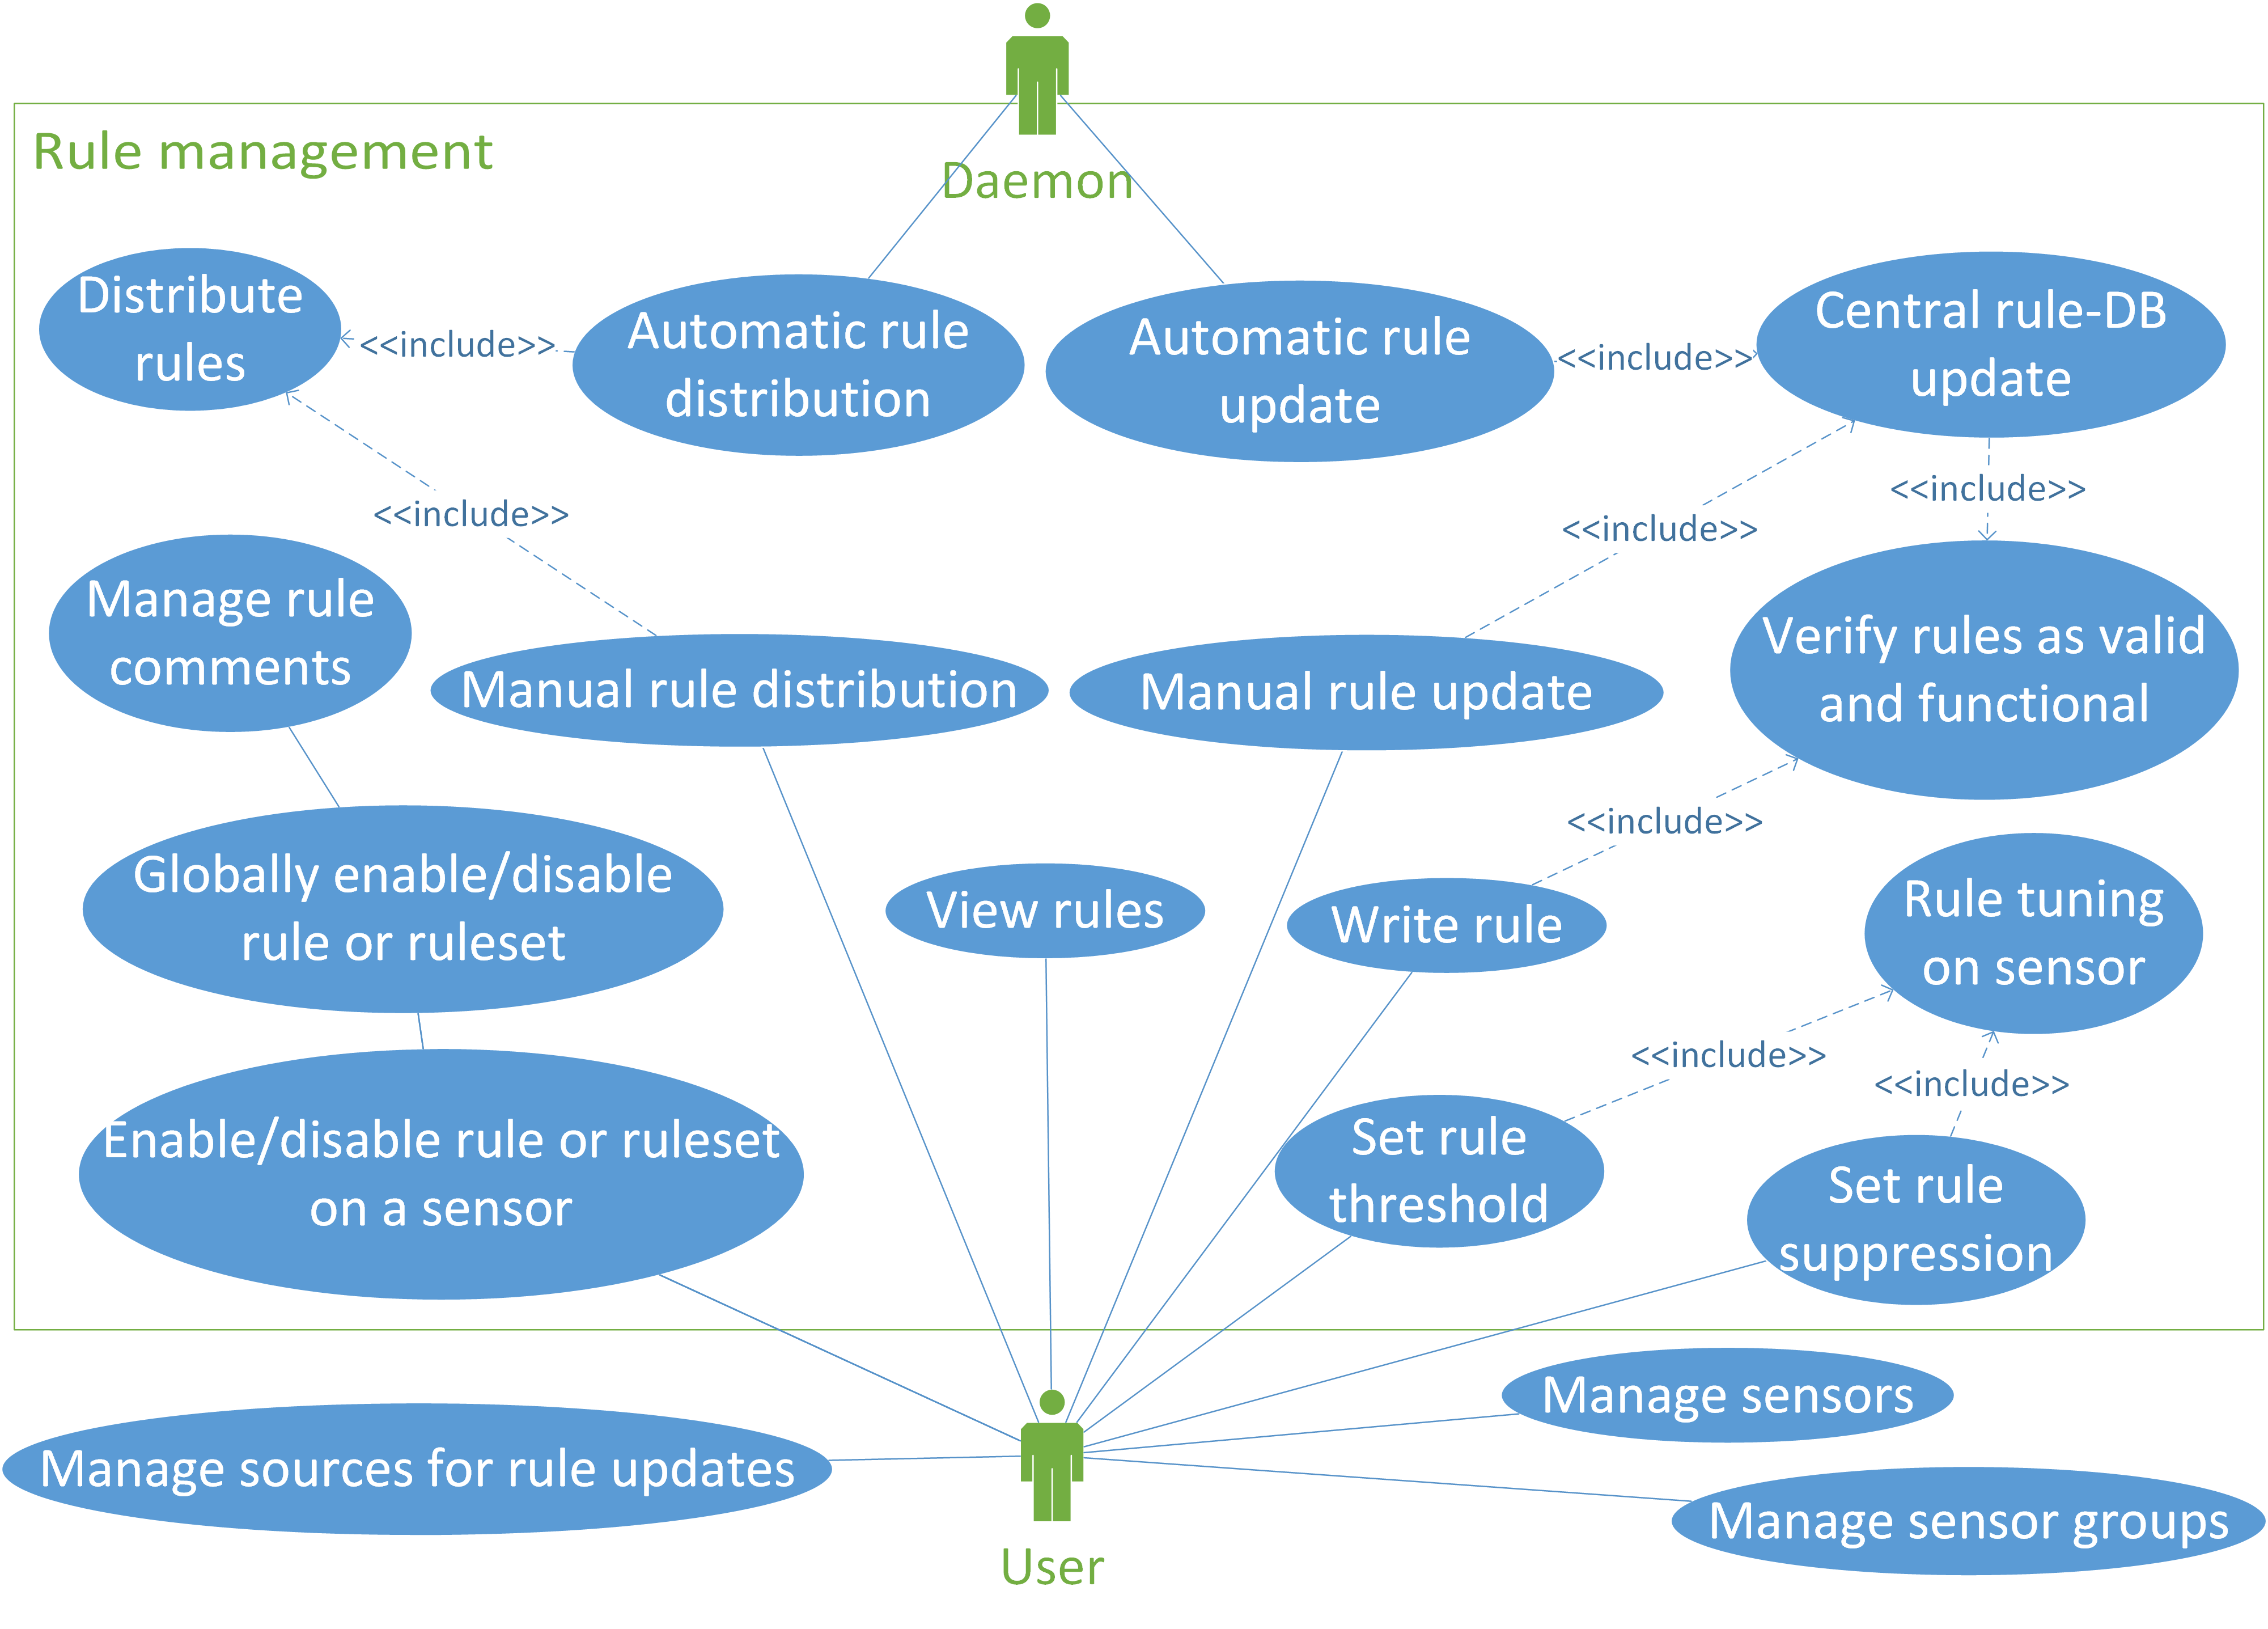
\includegraphics[width=200mm,angle=90]{./img/use-case-diagram-v2.png} 
\caption{Use case diagram}
\label{fig:use_case_diagram}
\end{figure}

\subsection{Domain Model}
After outlining all the concepts above, we created the conceptual class diagram
 in Figure \ref{fig:conceptual_class_diagram}, which shows the classes needed
in the system. Even though a \snort{} rule is quite simple by itself, there is a
lot of meta-information surrounding it, such as rule revisions and rule
classifications. Therefore, the system needed at least 16 different classes in
order to fullfil the basics of the required functionality.

\begin{figure}[!p]
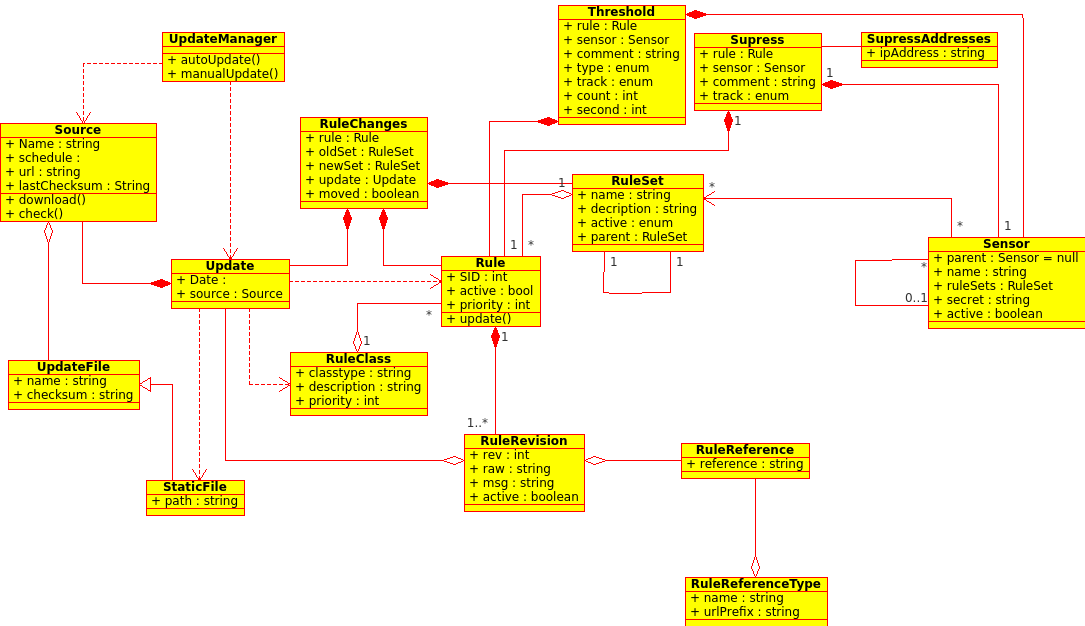
\includegraphics[width=200mm,angle=90]{./img/conceptual-class-diagram.png}
\caption{Conceptual class diagram}
\label{fig:conceptual_class_diagram}
\end{figure}

